%图表序号清零
\setcounter{table}{0}
\setcounter{figure}{0}

\subsection{\hei\xiaosan\textbf{参数优化}}

  不同于其他一些传统的\zs 黑盒机器学习方法,卷积网络\zs 所提取的
  图像特征在\zs 训练过程中是可视的,这不仅让人们对于卷积网络的工作过程
  有直观的了解,更能够帮助进行下一步的工作。在卷积网络的前向传播过程中\zs 
  部分卷积层滤波器提取的特征结果如图所示。

  \begin{figure}[H]
    \centering
    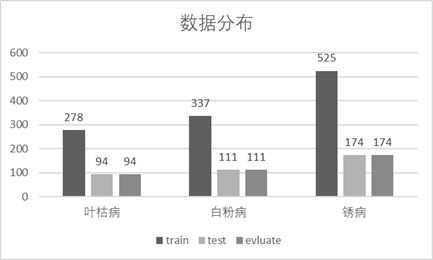
\includegraphics[width=.5\textwidth]{resource/数据分布.bmp}
    \caption{数据分布}
    \label{Figure.Fourth.1}
  \end{figure}

  为了改进本文模型的性能,在实验初期进行了不同迭代次数(分别为10000次、20000次)的实验,
  在图\ref{Figure.Fourth.2}中以[橙-深蓝]、[红-浅蓝]图像对应其测试集和验证集的准确率;而
  [粉-绿]图像代表了卷积网络初步优化后的效果。验证准确率在70\%\textasciitilde75\%徘徊的
  原因来自于数据集:因为数据来自百度和谷歌图库,而这些图片是从各个网页上收集而来,其中大
  多数含有水印且画质模糊,为了收集到足够的实验用数据集,便在粗略挑选、裁剪后应用于实验,
  故此准确率不高。

  第一次训练对应的是[橙-深蓝]图象。该图像是在初步建立卷积网络模型的情况下训练的,
  由于输入数据较为粗糙,准确率只有65\%左右。由\ref{Figure.Fourth.3}可以看出,
  在训练次数达到1500次时,验证损失率不降反升,这表明卷积网络模型存在过拟合的问题,
  而且在[红-浅蓝]图像中仍然存在该问题。[红-浅蓝]图像是训练了20000次的结果,在只有数据集
  稍微改进的情况下,验证准确率提升到72\%左右,但差别并不明显。

  在一些深度学习图像分类训练中,有的直接将测试集用作验证集,这可能有混淆概念的嫌疑。
  在调整数据集比例(训练集:测试集:验证集=3:1:1)后,又将输入图像的大小从
  $30\times30\times3$调整为$100\times100\times3$之后,便有了第三次的图像。
  从[粉-绿]图像可以明显看出,这次训练中用不到一千次迭代便将验证准确率提升至75\%,
  而测试准确率不到两千次便达到了99.84\%的准确率,远远好于前两次的训练效果。

  \begin{figure}[H]
    \centering
    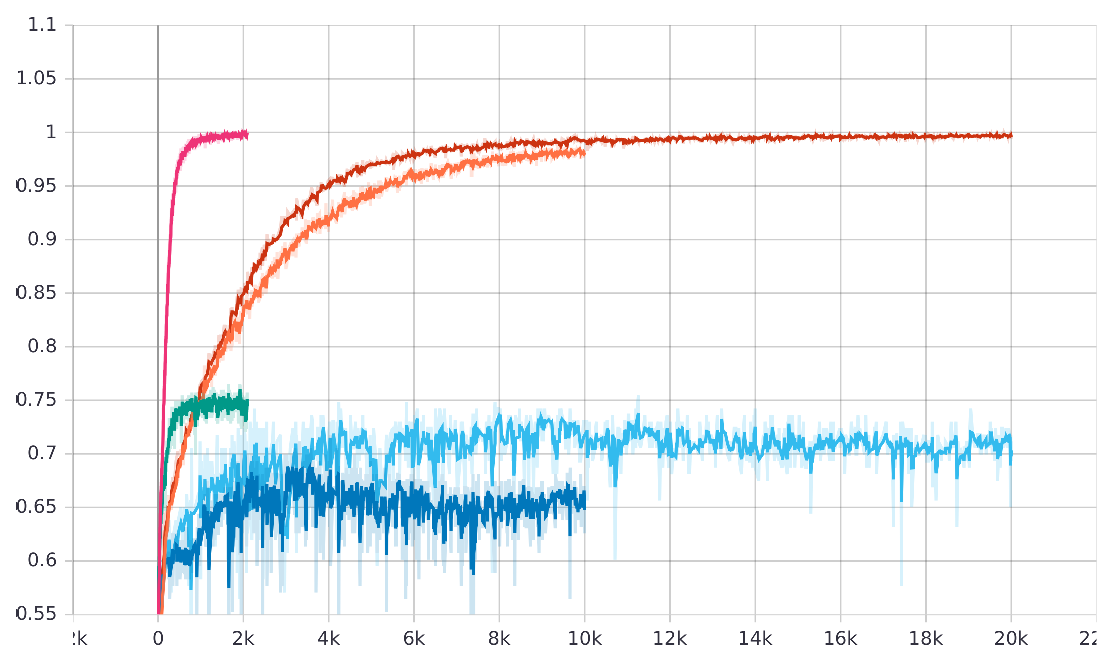
\includegraphics[width=.8\textwidth]{resource/epoch_accuracy.eps}
    \caption{训练-验证准确率}
    \label{Figure.Fourth.2}
  \end{figure}
  \begin{figure}[H]
    \centering
    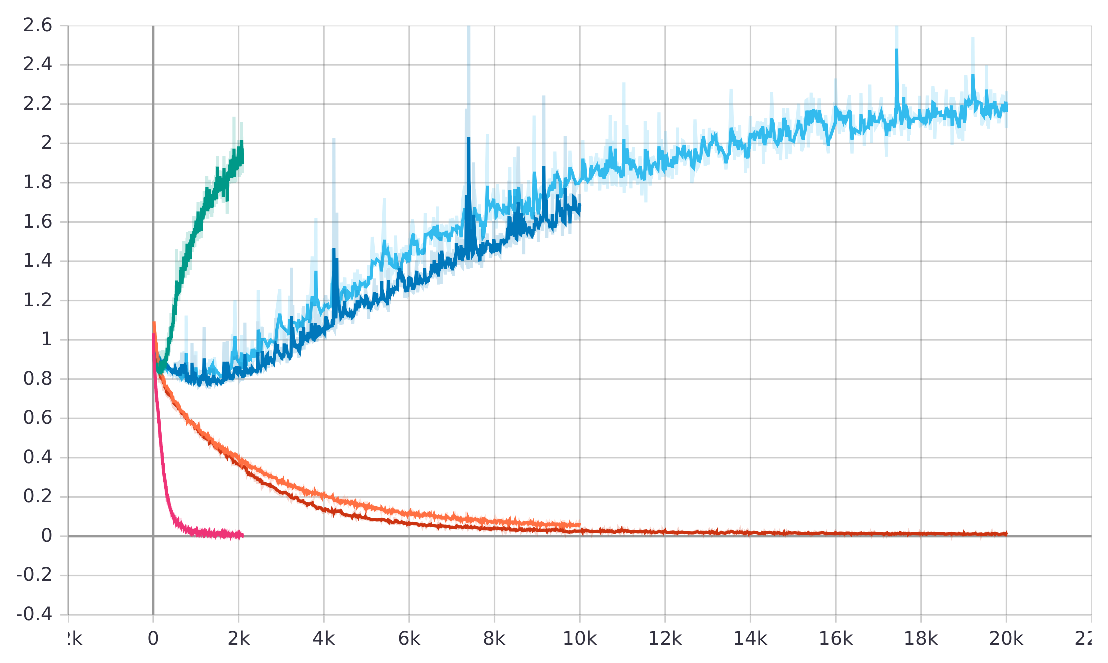
\includegraphics[width=.8\textwidth]{resource/epoch_loss.eps}
    \caption{训练-验证损失率}
    \label{Figure.Fourth.3}
  \end{figure}

% \subsection{\hei\xiaosan\textbf{模型对比}}
\subsection{\hei\xiaosan\textbf{实验总结}}
  本文提出了一种基于卷积神经网络的小麦病害识别方法。在初步建立该模型后,
  通过优化数据集、改进模型参数以减弱过拟合的影响等方面入手,通过多次实验得到了
  一个表现良好的小麦病害分类模型。
  后期将该模型与经典卷积网络模型LeNet-5、AlexNet等模型进行\zs 
  小麦病害识别对比实验,结果表明该模型具有更好的分类识别效果。